\documentclass{ctexart}

\usepackage{geometry}
\geometry {a4paper, scale = 0.8}
\usepackage{hyperref}
\usepackage{amsmath, amssymb, amsthm, mathtools}
% \numberwithin{equation}{section}                    % 定义公式的三级编号
\usepackage{comment}
\usepackage{tikz}
% \usepackage{xcolor}                                 % 引入定制颜色的xcolor
% \definecolor{LightBlue}{RGB}{226, 247, 254}         % 自定义颜色LightBlue
\usepackage{tcolorbox}
\tcbuselibrary{breakable, most, skins, theorems}
\newtcolorbox{question}[2][breakable] {
    colback = white,
    colframe = cyan, 
    fonttitle = \bfseries,  
    title = #2, #1
}
\newenvironment{solution}{\noindent{\textbf{{\color{cyan}解答}}}\quad}


% \usepackage[T1]{fontenc}                          % 敲入\dj显示\dbar
% \excludecomment{solution}                         % 编译此指令隐藏所有解答

\begin{document}
\title{《热力学·统计物理》习题}
\author{郑锦阳}
\date{\today}
\maketitle
\tableofcontents
\section{热力学的基本规律}

\begin{question}{题目1.1}
    试求理想气体的体胀系数$\alpha$,压强系数$\beta$ 和等温压缩系数 $\kappa_T$.
\end{question}
\begin{solution}
    对理想气体状态方程两边取偏微分
    $$
        V\,\partial{p}+p\,\partial{V}=\nu R\,\partial{T}
    $$
    体胀系数$\alpha$
    $$
        \alpha=\frac{1}{V}\left(\frac{\partial V}{\partial T}\right)_p
        =\frac{1}{V}\frac{\nu R}{p}
        =\frac{1}{T}
    $$
    压强系数$\beta$
    $$
        \beta=\frac{1}{p}\left(\frac{\partial p}{\partial T}\right)_V
        =\frac{1}{p}\frac{\nu R}{V}
        =\frac{1}{T}
    $$
    等温压缩系数$\kappa_T$
    $$
        \kappa_T=-\frac{1}{V}\left(\frac{\partial V}{\partial p}\right)_T
        =-\frac{1}{V}\left(-\frac{V}{p}\right)
        =\frac{1}{p}
    $$
\end{solution}



\begin{question}{题目1.2}
    试证明:对于任意一种具有两个独立参量$T,p$的物质,如果通过实验测得其体胀系数$\alpha$及等温压缩系数$\kappa_T$,那么它的物态方程必定可以通过下述积分求得
    \begin{equation}\label{物态方程的积分形式}
        \ln{V}=\int(\alpha\,\mathrm{d}T-\kappa_T\,\mathrm{d}p)
    \end{equation}
    如果$\alpha=\dfrac{1}{T}$,$\kappa_T=\dfrac{1}{p}$,试求物态方程.
\end{question}
\begin{solution}
    (1) 根据体胀系数$\alpha$和等温压缩系数$\kappa_T$的定义,积分化为
    $$
        \ln{V}=\int\frac{1}{V}\left(\frac{\partial V}{\partial T}\right)_p\mathrm{d}T-\left(-\frac{1}{V}\right)\left(\frac{\partial V}{\partial p}\right)_p\mathrm{d}p
        =\int\frac{1}{V}\left[\left(\frac{\partial V}{\partial T}\right)_p\mathrm{d}T+\left(\frac{\partial V}{\partial p}\right)_p\mathrm{d}p\right]
    $$
    由于$T,p$两个参量相互独立,所以中括号内的表达式恰好是$V(T,p)$的全微分
    $$
        \ln{V}=\int\frac{1}{V}\,\mathrm{d}V\equiv\ln{V}
    $$
    (2) 如果我们代入已知条件$\alpha=\cfrac{1}{T}$,$T=\cfrac{1}{p}$
    $$
        \ln{V}
        =\int\left(\frac{1}{T}\,\mathrm{d}T-\frac{1}{p}\,\mathrm{d}p\right)
        =\ln{T}-\ln{p}+C
    $$
    化简得到
    $$
        pV=CT \quad (C>0)
    $$
\end{solution}


\begin{question}{题目1.4}
    在0℃和1atm下,测得一铜块的体胀系数和等温压缩系数分别为$\alpha=4.85\times10^{-5}\,\mathrm{K^{-1}}$和$\kappa_T=7.8\times10^{-7}\rm{atm^{-1}}$. $\alpha$和$\kappa_T$可近似看作常量. 现将铜块加热至10℃. 问:
    \begin{enumerate}
        \item 压强要增加到多少才能使铜块的体积维持不变?
        \item 若压强增加到100atm,铜块的体积改变多少?
    \end{enumerate}
\end{question}
\begin{solution}
    根据此前已证明的物态方程$\eqref{物态方程的积分形式}$
    \begin{equation}\label{物态方程的微分形式}
        \frac{1}{V}\,\mathrm{d}V=\alpha\,\mathrm{d}T-\kappa_T\,\mathrm{d}p
    \end{equation}
    (1) 加压能够完全抑制铜块的体积变化,所以$\mathrm{d}V=0$
    $$
        \Delta{p}
        =\frac{\alpha}{\kappa_T}\Delta{T}
        =\frac{4.85\times 10^{-5}}{7.8\times 10^{-7}}\times 10
        =622 {\,\rm Pa}
    $$
    (2) 铜块的体积随压强和温度变化,所以
    $$
        \frac{\Delta{V}}{V}
        =\alpha\Delta{T}-\kappa_T\Delta{p}
        =4.85 \times 10^{-5} \times 10 - 7.8 \times 10^{-7} \times 99
        =4.07 \times 10^{-4}
    $$
\end{solution}


\begin{question}{题目1.7}
    抽成真空的小匣带有活门,打开活门让气体冲入. 当压强达到外界压强$p_0$时将活门关上. 试证明:小匣内的空气在没有与外界交换热量之前,它的内能$U$与原来在大气中的内能$U_0$之差为$U-U_0=p_0V_0$,其中$V_0$是它原来在大气中的体积. 若气体是理想气体,求它的温度和体积.
\end{question}
\begin{solution}
    (1) 根据热力学第二定律
    $$
        U-U_0=W+Q
    $$
    由于过程迅速,可以认为系统与外界没有热量交换,即
    $$
        Q=0
    $$
    且只有外界对系统等压做功,而小匣对外界涌入的气体无阻碍作用
    $$
        W=p_0V_0
    $$
    所以
    $$
        U-U_0=p_0V_0
    $$
    (2) 如果气体是理想气体,则满足理想气体状态方程
    $$
        p_0V_0=nRT_0
    $$
    和
    $$
        C_V=\frac{nR}{\gamma-1}, \quad C_p=\gamma\frac{nR}{\gamma-1}, \quad U=\int_{}^{}C_V\,\mathrm{d}T
    $$
    所以
    $$
        U-U_0
    $$
\end{solution}


\begin{question}{题目1.8}
    满足$pV^n=C$(常量)的过程称为多方过程,其中常数$n$称为多方指数. 试证明:理想气体在多方过程中的热容$C_n=\cfrac{n-\gamma}{n-1}C_V$
\end{question}
\begin{solution}
    多方过程的热容为
    $$
        C_n=\lim_{\Delta{T}\to0}\left(\frac{\Delta Q}{\Delta T}\right)_n
        =\lim_{\Delta{T}\to0}\left(\frac{\Delta U+p\Delta V}{\Delta T}\right)_n
        = \left(\frac{\partial U}{\partial T}\right)_n+p\left(\frac{\partial V}{\partial T}\right)_n
    $$
    理想气体的内能只与温度有关
    $$
        C_V = \left(\frac{\partial U}{\partial T} \right)_n
    $$
    再对多方过程方程两边取全微分
    $$
        V^{n-1}\,\mathrm{d}T+(n-1)V^{n-2}T\,\mathrm{d}V=0
    $$
    结合理想气体状态方程得到
    $$
        \left(\frac{\partial V}{\partial T}\right)_n = \frac{V}{(n-1)T}
    $$
    最终
    $$
        C_n=C_V-\frac{pV}{T(n-1)}=\frac{n-\gamma}{n-1}C_V
    $$
\end{solution}


\begin{question}{题目1.9}
    假设气体的定压热容和定容热容是常量,试证明:若理想气体在某一过程中的热容$C_n$是常量,则该过程一定是多方过程,且多方指数为$n=\cfrac{C_n-C_p}{C_n-C_V}$
\end{question}
\begin{solution}
    根据热力学第一定律
    $$
        C_V\,\mathrm{d}T=C_n\,\mathrm{d}T-p\,\mathrm{d}V
    $$
    利用理想气体的物态方程消去$p$并结合$C_p-C_V=nR$
    $$
        (C_n-C_V)\frac{\mathrm{d}T}{T}=(C_p-C_V)\frac{\mathrm{d}V}{V}
    $$
    进一步,利用理想气体状态方程的微分形式
    $$
        \frac{\mathrm{d}p}{p}+\frac{\mathrm{d}V}{V}=\frac{\mathrm{d}T}{T}
    $$
    消去$T$
    $$
        (C_n-C_V)\frac{\mathrm{d}p}{p}-(C_n-C_p)\frac{\mathrm{d}V}{V}=0
    $$
\end{solution}


\begin{question}{题目1.16}
    理想气体分别经等压过程和等容过程,温度由$T_1$升至$T_2$. 假设$\gamma$是常数,试证明前者的熵增为后者的$\gamma$倍.
\end{question}
\begin{solution}
    等压过程的熵增为
    $$
        \Delta{S_1}=C_p\ln\frac{T_2}{T_2}
    $$
    等同过程的熵增为
    $$
        \Delta{S_2}=C_V\ln\frac{T_2}{T_2}
    $$
    所以
    $$
        \gamma=\frac{\Delta{S_1}}{\Delta{S_2}}=\frac{C_p}{C_V}
    $$
\end{solution}


\begin{question}{题目1.19}
    均匀杆的温度一端为$T_1$,另一端为$T_2$. 试计算达到均匀温度$\cfrac12(T_1+T_2)$后的熵增.
\end{question}
\begin{solution}
\end{solution}


\begin{question}{题目1.21}
    物体的初温$T_1$高于热源的温度$T_2$. 有一热机在此物体与热源之间工作,直到将物体的温度降低到$T_2$为止. 若热机从物体吸取的热量为$Q$,试根据熵增加原理证明:此热机所能输出的最大功为
    $$
        W_{\max}=Q-T_2(S_1-S_2)
    $$
    其中$S_1-S_2$是物体的熵变.
\end{question}
\begin{solution}
\end{solution}


\begin{question}{题目1.23}
    简单系统有两个独立参量. 如果以$T,S$为独立参量,可用纵坐标表示温度$T$,横坐标表示熵$S$,构成$T-S$图. 图中的一点与系统的一个平衡态相对应,一条曲线与一个可逆过程相对应. 试在图中画出可逆卡诺循环过程的曲线,并利用$T-S$图求卡诺循环的效率.
\end{question}
\begin{solution}
\end{solution}
\section{均匀介质的热力学性质}
\subsection{内能、焓、自由能和吉布斯函数的全微分}
热力学函数的全微分助记符如下:
\begin{center}
    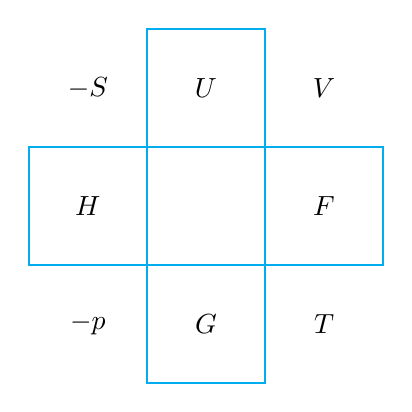
\begin{tikzpicture}[scale=1.5]
        \node at (0, -1) {$G$};
        \node at (-1, 0) {$H$};
        \node at (0, +1) {$U$};
        \node at (+1, 0) {$F$};
        \draw[cyan, thick] (-0.5, 1.5) rectangle (0.5, -1.5);
        \draw[cyan, thick] (-1.5, -0.5) rectangle (1.5, 0.5);
        \node at (-1, -1) {$-p$};
        \node at (-1, +1) {$-S$};
        \node at (+1, +1) {$V$};
        \node at (+1, -1) {$T$};
    \end{tikzpicture}
\end{center}
每个热力学函数的两边是其微分项(无需考虑正负号),而微分项对角线位置正好是各微分项对应的线性主部(需要考虑正负号). 以吉布斯函数$G$为例,其两边是微分项$\mathrm{d}p$和$\mathrm{d}T$,微分项的对角线位置是各自的线性主部$V$和$-S$,于是
$$
    \mathrm{d}G = V\mathrm{d}p - S\mathrm{d}T
$$
然后依次导出各热力学函数的全微分
\begin{equation}\label{吉布斯函数的全微分}
    \mathrm{d}G = V\mathrm{d}p - S\mathrm{d}T
\end{equation}
\begin{equation}\label{焓的全微分}
    \mathrm{d}H = T\mathrm{d}S - V\mathrm{d}p
\end{equation}
\begin{equation}\label{内能的全微分}
    \mathrm{d}U = T\mathrm{d}S - p\mathrm{d}V
\end{equation}
\begin{equation}\label{自由能的全微分}
    \mathrm{d}F = -p\mathrm{d}V - S\mathrm{d}T
\end{equation}



\subsection{麦克斯韦关系}
下面以吉布斯函数$G$为例,介绍各个热力学函数的麦克斯韦关系:首先根据吉布斯函数的全微分,写出其偏导数
$$
    \left(\frac{\partial G}{\partial p}\right)_T=V, \quad
    \left(\frac{\partial G}{\partial T}\right)_p=-S,
$$
由于$G$是连续函数,所以它的二阶混合偏导数必然相等
$$
    \left[\frac{\partial}{\partial T}\left(\frac{\partial G}{\partial p}\right)_T\right]_p = -\left[\frac{\partial}{\partial p}\left(\frac{\partial G}{\partial T}\right)_p\right]_T
$$
也即
$$
    -\left(\frac{\partial S}{\partial p}\right)_T=\left(\frac{\partial V}{\partial T}\right)_p
$$
类似地,我们能依次导出所有热力学函数的麦克斯韦关系
\begin{align}\label{麦克斯韦关系}
    -\left(\frac{\partial S}{\partial p}\right)_T & = \left(\frac{\partial V}{\partial T}\right)_p  \\
    \left(\frac{\partial T}{\partial p}\right)_S  & = \left(\frac{\partial V}{\partial S}\right)_p  \\
    \left(\frac{\partial T}{\partial V}\right)_S  & = -\left(\frac{\partial p}{\partial S}\right)_V \\
    \left(\frac{\partial p}{\partial T}\right)_V  & = \left(\frac{\partial S}{\partial V}\right)_T
\end{align}
这一切操作和变换,都是为了把无法通过实验直接测量的热力学函数$G, H, U, F$转化为可以通过实验直接测量的参量$p, S, V, T$.



\subsection{气体的节流过程和绝热膨胀过程}
\paragraph{节流过程}管子用不导热的材料制成,管子中间有一个多孔塞,多孔塞两边各维持着较高的压强$p_1$和较低的压强$p_2$,于是气体从高压的一边经过多孔塞不断地流向低压的一边,并达到定常状态.


\subsection{基本热力学函数的确定}
\section{热力学·统计物理2023年第二学期期末}

\subsection{填空题(每小题3分,共6小题,计18分)}
\begin{question}{题目1}
    1mol理想气体的物态方程为\underline{\qquad}\underline{\qquad}
\end{question}

\begin{question}{题目2}
    当系统在恒定的外界压强$p$下体积由$V_1$变为$V_2$时,外界对系统所做的功为$W=$\underline{\qquad}\underline{\qquad}
\end{question}

\begin{question}{题目3}
    在等温等容的条件下,系统的\underline{\qquad}\underline{\qquad}永不增加
\end{question}

\begin{question}{题目4}
    某系统有两个能级,第一个能级有三个量子态,第二个能级有两个量子态。系统由四个全同的玻色子组成,则两个粒子处于第一能级、两个粒子处于第二能级的微观状态数为\underline{\qquad}\underline{\qquad}
\end{question}

\begin{question}{题目5}
    由能量均分定理可知,温度为$T$时的$N$个弹性双原子分子组成的理想气体的内能是\underline{\qquad}\underline{\qquad}
\end{question}

\begin{question}{题目6}
    假设系统有20个全同粒子组成,粒子的自由度为3,则系统的自由度为\underline{\qquad}\underline{\qquad}
\end{question}


\subsection{简答题(每小题6分,共2小题,计12分)}
\begin{question}{题目1}
    对于等温等压系统,通常选择的特性函数是什么?为什么?
\end{question}

\begin{question}{题目2}
    正则系统适用于讨论粒子数、能量、体积一定的孤立系统。以上说法是否正确?为什么?
\end{question}

\subsection{推导证明题(每小题12分,共3小题,计36分)}
\begin{question}{题目1}
    能态方程给出了在温度保持不变时内能随体积的变化率与物态方程之间的关系,试推导之。
\end{question}

\begin{question}{题目2}
    试推导Fermi分布$\displaystyle a_l=\frac{\omega_l}{\mathrm{e}^{\alpha+\beta\varepsilon_l}+1}$
\end{question}

\begin{question}{题目3}
    试推导Bose统计中描述系统状态的参量$p$的统计表达式(即它与巨配分函数的关系)
\end{question}


\subsection{计算题(共3小题,计34分)}
\begin{question}{题目1}
    焦汤系数表示在焓不变的条件下,气体温度随压强的变化率。试求气体在节流膨胀过程中的焦汤系数。
\end{question}
\begin{question}{题目2}
    一维线性谐振子能量的经典表达式为
    $$
        \varepsilon=\frac{p^2}{2m}+\frac{1}{2}m\omega^2q^2
    $$
    试计算经典近似的谐振子配分函数及内能。
\end{question}
\begin{question}{题目3}
    试求绝对零度下自由电子气体中电子的平均速率。
\end{question}


\end{document}